\documentclass{beamer}
\usetheme{Malmoe}

\usepackage{graphicx}
\usepackage{minted}
\usepackage{xcolor}
\usepackage{tikz}
\usetikzlibrary{positioning,shapes,shadows,arrows}
\tikzstyle{object}=[rectangle, draw=black, rounded corners, fill=blue!40, drop shadow,
        text centered, anchor=north, text=white, text width=3cm]
\tikzstyle{highlight}=[rectangle, draw=black, rounded corners, fill=red!40, drop shadow,
        text centered, anchor=north, text=white, text width=3cm]

\tikzstyle{comment}=[rectangle, draw=black, rounded corners, fill=white, drop shadow,
        text centered, anchor=north, text=black, text width=3cm]

\title{From 0 to DIY Web App in 120 minutes}
\author[daniel@axtens.net]{Daniel Axtens\\daniel@axtens.net\\@daxtens}

\newcommand\aws[1]{\textcolor{purple}{\texttt{#1}}}

\begin{document}

% -------------------------------------------
\begin{frame}[plain]
  \titlepage
\end{frame}


\begin{frame}
  \frametitle{Outline}
  \tableofcontents
\end{frame}

% -------------------------------------------

\section{Getting Started}

\begin{frame}
  \frametitle{When you should not use this}
  \begin{itemize}
  \item Static web site $\to$ static HTML and CSS.
  \item User-editable content --- blog/corporate website $\to$ Content Managment System
  \item Data driven and highly structured data, well understood
    system based around Create Retrieve Update Delete (CRUD) $\to$
    e.g. Django
  \end{itemize}
\end{frame}

\begin{frame}
  \frametitle{When you should use this}
  \begin{itemize}
  \item Something requiring persistent storage but where the data is
    not highly structured, or has a frequently changing schema or is
    otherwise difficult to reduce to a relational database $\to$ a
    non-relational database (NoSQL): e.g. MongoDB
  \item Something so small that setting up something like Django will
    take longer than actually implementing the functionality $\to$ a
    micro-framework, e.g. Bottle
  \end{itemize}
\end{frame}

\begin{frame}
  \frametitle{Start thinking...}
  \begin{itemize}
  \item There's no set end product for this workshop. There will be
    several spots where you can decide for yourself what to do, and
    get assistance in making it happen.

  \item Start thinking about a (relatively) simple application that
    (preferably) fits the previous critera, or at least is dynamic
    with persistent storage. Perhaps:
    \begin{itemize}
    \item Collate information from a variety of internet-connected
      sensors, process it, and display a
      result. (e.g. average/min/max?)
    \item A database of quotable quotes, with up/down-voting
    \item Configurable Insult/3 word slogan/etc
      generator
    \item Your idea here.
    \item Really stuck? (Yet another) blog with comments, photo-sharing service,
      todo list, calendar, social-bookmarking service, etc. (Most of
      these things are better built with e.g. Django)
    \end{itemize}
  \end{itemize}
\end{frame}

\begin{frame}
  \frametitle{Get on the internet}
  \begin{itemize}
  \item Get on the internet.

  \item Go to \\\url{http://dja.compcon.dja.id.au/static/presentation.pdf}\\ to get these instructions so you
    can follow along at your own pace!
  \end{itemize}
\end{frame}


\begin{frame}
  \frametitle{Local environment}
  \begin{itemize}
  \item Set up git to point this to your repository, not mine.
    \begin{itemize}
    \item Fork the repo on GitHub.
    \item \texttt{git remote set-url origin
        https://github.com/\textit{YOU}/diy-web-app}
    \item (Unless you already have private keys set up, in which case
      use \texttt{git@github.com:\textit{YOU}/diy-web-app.git})
    \end{itemize}
  \item \texttt{vagrant up}
  \item \texttt{vagrant ssh}
  \item Any changes you make to your local file system are reflected in the virtual machine in the \texttt{/vagrant} directory.
  \end{itemize}
\end{frame}

\begin{frame}
  \frametitle{Remote environment}
  
  \begin{itemize}
  \item You get a week of EC2 time on AWS to build/experiment with your app.
  \item AWS (Amazon Web Services) $\to$ a set of services.
    \begin{itemize}
    \item EC2 - Elastic Cloud Compute $\to$ Virtual Machines
    \item SES - Simple Email Service
    \item Route 53 - DNS service $\to$ maps names like google.com to
      IP addresses like 203.8.182.219
    \item S3 - Simple Storage Service $\to$ Way to store static assets/files.
    \item CloudFront - CDN (Content Delivery Network) $\to$ caches
      static assets near the user for faster speed, less load on your
      server.
    \item And many, many more.
    \end{itemize}
  \item Not free in general, but a free tier exists.
  \end{itemize}
\end{frame}

\begin{frame}
  \frametitle{Remote Environment}
  \begin{itemize}
  \item You should have a bit of paper with the details of your EC2
    instance.
  \item Follow those instructions. You should end up with a shell
    on your EC2 instance.
  \item Update the package lists and packages: \aws{sudo apt-get
      update; sudo apt-get -y upgrade; sudo reboot}
  \item SSH in again after it reboots.
  \end{itemize}
\end{frame}

\subsection{Anatomy of a simple web app}

\subsubsection{Overview}

\begin{frame}
  \frametitle{Anatomy of a simple web app: overview}

  \begin{center}
    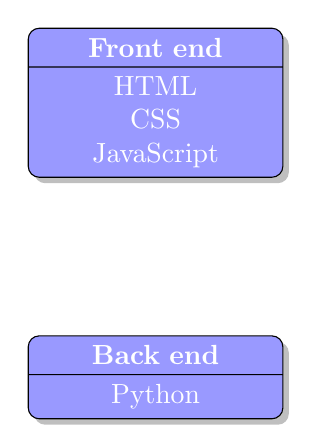
\begin{tikzpicture}[node distance=2cm]
      \node (Frontend) [object, rectangle split, rectangle split parts=2]
      {
        \textbf{Front end}
        \nodepart{second}HTML \\ CSS \\ JavaScript
      };
      \node (Backend) [object, rectangle split, rectangle split parts=2, below=of Frontend]
      {
        \textbf{Back end}
        \nodepart{second}Python
      };
    \end{tikzpicture}
  \end{center}
\end{frame} 

\begin{frame}
  \frametitle{Anatomy of a simple web app: now add a database}
  \begin{center}
      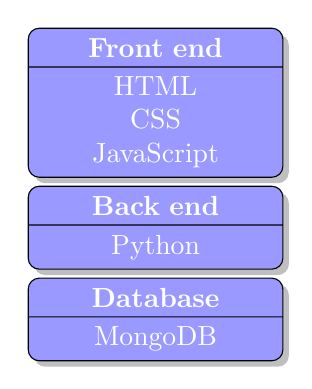
\begin{tikzpicture}[node distance=2cm]
        \node (Frontend) [object, rectangle split, rectangle split parts=2]
        {
          \textbf{Front end}
          \nodepart{second}HTML \\ CSS \\ JavaScript
        };
        \node (Backend) [object, rectangle split, rectangle split parts=2, below=0.1cm of Frontend]
        {
          \textbf{Back end}
          \nodepart{second}Python
        };
        \node (Database) [object, rectangle split, rectangle split parts=2, below=0.1cm of Backend]
        {
          \textbf{Database}
          \nodepart{second}MongoDB
        };
      \end{tikzpicture}
    \end{center}
\end{frame}

\subsubsection{Delivery}

\begin{frame}
  \frametitle{Anatomy of a simple web app: how does this get to you?}
  \framesubtitle{Ideal world}
  \begin{center}
      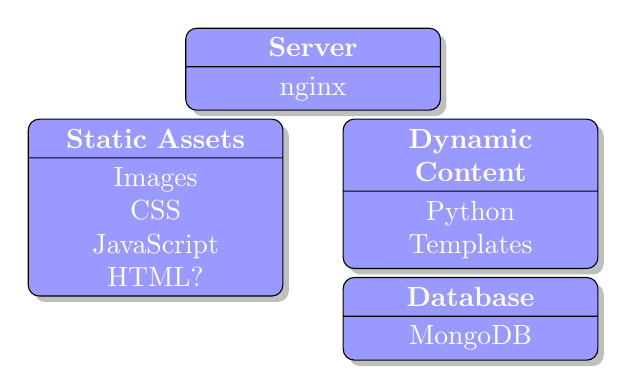
\begin{tikzpicture}[node distance=0.1cm]
        \node (Server) [object, rectangle split, rectangle split parts=2]
        {
          \textbf{Server}
          \nodepart{second}nginx
        };
        \node (Frontend) [object, rectangle split, rectangle split parts=2, below=of Server, xshift=-2cm]
        {
          \textbf{Static Assets}
          \nodepart{second}Images \\ CSS \\ JavaScript \\HTML?
        };
        \node (Backend) [object, rectangle split, rectangle split parts=2, below=of Server, xshift = 2cm]
        {
          \textbf{Dynamic Content}
          \nodepart{second}Python\\Templates
        };
        \node (Database) [object, rectangle split, rectangle split parts=2, below=of Backend]
        {
          \textbf{Database}
          \nodepart{second}MongoDB
        };
      \end{tikzpicture}
    \end{center}
\end{frame}

\begin{frame}
  \frametitle{Anatomy of a simple web app: how does this get to you?}
  \framesubtitle{Our world}
  \begin{center}
      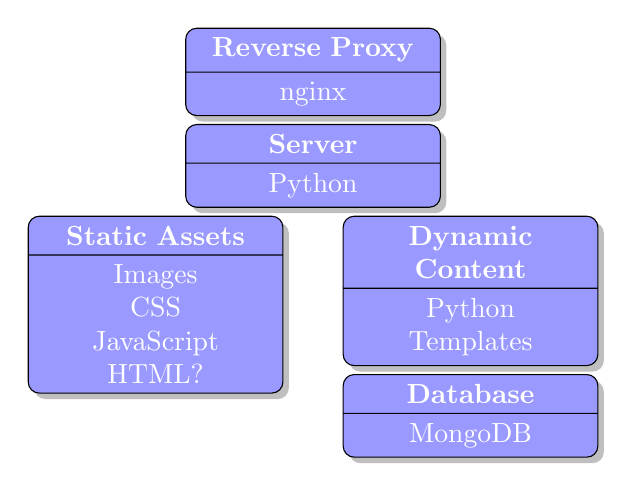
\begin{tikzpicture}[node distance=0.1cm]
        \node (proxy) [object, rectangle split, rectangle split parts=2]
        {
          \textbf{Reverse Proxy}
          \nodepart{second}nginx
        };
        \node (Server) [object, rectangle split, rectangle split parts=2, below=of proxy]
        {
          \textbf{Server}
          \nodepart{second}Python
        };
        \node (Frontend) [object, rectangle split, rectangle split parts=2, below=of Server, xshift=-2cm]
        {
          \textbf{Static Assets}
          \nodepart{second}Images \\ CSS \\ JavaScript \\ HTML?
        };
        \node (Backend) [object, rectangle split, rectangle split parts=2, below=of Server, xshift = 2cm]
        {
          \textbf{Dynamic Content}
          \nodepart{second}Python\\Templates
        };
        \node (Database) [object, rectangle split, rectangle split parts=2, below=of Backend]
        {
          \textbf{Database}
          \nodepart{second}MongoDB
        };
      \end{tikzpicture}
    \end{center}
\end{frame}

\section{Building your app}

\begin{frame}
  \frametitle{Building your app}
\end{frame}

\subsection{Server}

\begin{frame}
  \frametitle{Server}
    \begin{center}
      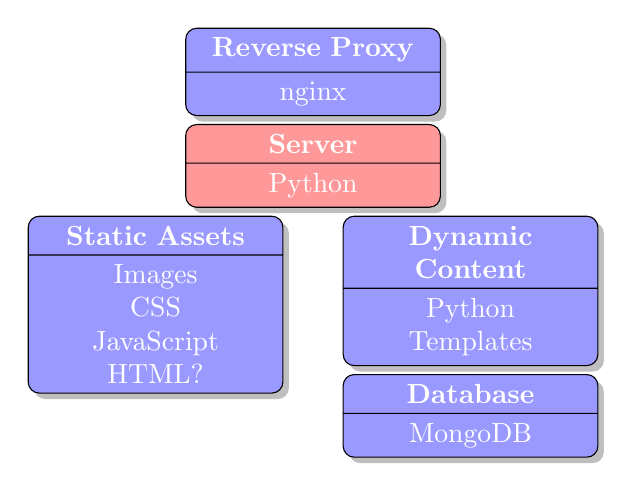
\begin{tikzpicture}[node distance=0.1cm]
        \node (proxy) [object, rectangle split, rectangle split parts=2]
        {
          \textbf{Reverse Proxy}
          \nodepart{second}nginx
        };
        \node (Server) [highlight, rectangle split, rectangle split parts=2, below=of proxy]
        {
          \textbf{Server}
          \nodepart{second}Python
        };
        \node (Frontend) [object, rectangle split, rectangle split parts=2, below=of Server, xshift=-2cm]
        {
          \textbf{Static Assets}
          \nodepart{second}Images \\ CSS \\ JavaScript \\ HTML?
        };
        \node (Backend) [object, rectangle split, rectangle split parts=2, below=of Server, xshift = 2cm]
        {
          \textbf{Dynamic Content}
          \nodepart{second}Python\\Templates
        };
        \node (Database) [object, rectangle split, rectangle split parts=2, below=of Backend]
        {
          \textbf{Database}
          \nodepart{second}MongoDB
        };
      \end{tikzpicture}
    \end{center}
\end{frame}

\begin{frame}
  \frametitle{Introducing Bottle}
  \begin{figure}[h!]
    \centering
    
\includegraphics{imgs/bottle_logo}
    \caption{Bottle is a fast, simple and lightweight WSGI micro web-framework for Python. \url{http://bottlepy.org/}}
    \label{fig:bottle_logo}
  \end{figure}

  You might also want to consider Flask: \url{http://flask.pocoo.org/}. It does a bit more for you/has a bit more magic than Bottle.

\end{frame}

\begin{frame}
  \frametitle{Hello World!}
  Edit \texttt{webapp.py}.
\hrule
  \inputminted{python}{../steps/01-hello-world/01-webapp.py}
\hrule
In your vagrant shell, \texttt{cd /vagrant; python webapp.py}.

Then visit \url{http://localhost:8080} in your browser.
\end{frame}

\begin{frame}
\frametitle{Best practices: commit your changes!}
\texttt{git add webapp.py}\\
\texttt{git commit -m"Hello world example"}\\
\texttt{git push}
\end{frame}

\begin{frame}[fragile]
  \frametitle{Greeting others}
  Let's extend:
  \begin{minted}{python}
@route('/greet/<name>')
def greet(name):
    return "Hello, %s!" % name
  \end{minted}

  \hrule
  \texttt{git add webapp.py}\\
  \texttt{git commit -m"Add greet function"}\\
  \texttt{git push}
\end{frame}

\begin{frame}
  \frametitle{Danger, Will Robinson!}
  Spot the subtle error and potential security hole.
\end{frame}

\begin{frame}
  \frametitle{Danger, Will Robinson!}

  What happens if you go to \url{localhost:8080/greet/<b>Daniel}?

  \textbf{This unescaped HTML has the potential (in other
    circumstances) to cause XSS vulnerabilites.}

  Fortunately, it's easy to avoid.
\end{frame}

\begin{frame}[fragile]
  \frametitle{Safe user input the right way}
  
  {\large Don't try to sanitise it yourself.}

  You will probably miss an edge case.

  \vskip1em

  {\Large Use templates.}

  \begin{minted}{python}
    from bottle import route, run, template

    ...

    def greet(name):
    	return template("Hello, {{name}}!", name=name)
  \end{minted}

\end{frame}

\begin{frame}[fragile]
  \frametitle{Separating presentation and content}
  We don't want template code in \texttt{.py} files.

  Edit \texttt{views/hello.tpl}. Fill it with standard HTML, with
  \texttt{\{\{name\}\}} somewhere. (Lazy? See the link to the sample
  on the notes.)

  Then:
  \begin{minted}{python}
    from bottle import route, run, template, view

    ...

    @route('/greet/<name>')
    @view('hello')
    def greet(name):
    	return {'name': name}
  \end{minted}

  \textbf{Bottle's template language (SimpleTemplate Engine) has more
    features, which we'll cover later...}
\end{frame}

\begin{frame}[fragile]
  \frametitle{Simplifying things}
  Why do we have different functions for \texttt{/} and \texttt{/greet}, when they do
  mostly the same thing? \textbf{A bottle function can handle multiple
  routes.}

  \begin{minted}{python}
@route('/')
@route('/greet/<name>')
@view('hello')
def greet(name="World"):
  \end{minted}
\end{frame}

\begin{frame}
\frametitle{Best practices: commit your changes!}
\texttt{git add webapp.py views/hello.tpl}\\
\texttt{git commit -m"Serve Hello World with a template."}\\
\texttt{git push}
\end{frame}


\begin{frame}[fragile]
  \frametitle{Serving static files}
  \textcolor{red}{\large Put them in a separate sub-directory!}

  \begin{minted}{python}
from bottle import route, run, template, view, static_file
import os

root = os.path.dirname(__file__)
static_root = os.path.join(root, "static")

...

@route('/static/<path:path>')
def static(path):
    return static_file(path, root=static_root)
    \end{minted}
\end{frame}

\begin{frame}
\frametitle{Best practices: commit your changes!}
\texttt{git add webapp.py}\\
\texttt{git commit -m"Serve static files out of static/"}\\
\texttt{git push}
\end{frame}

\begin{frame}
  \frametitle{Server}
    \begin{center}
      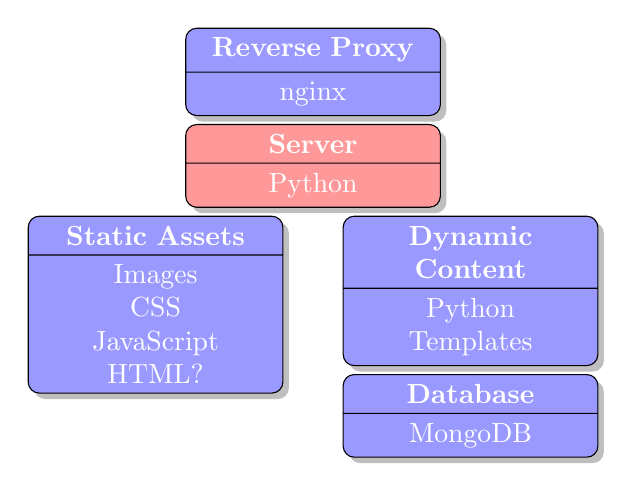
\begin{tikzpicture}[node distance=0.1cm]
        \node (proxy) [object, rectangle split, rectangle split parts=2]
        {
          \textbf{Reverse Proxy}
          \nodepart{second}nginx
        };
        \node (Server) [highlight, rectangle split, rectangle split parts=2, below=of proxy]
        {
          \textbf{Server}
          \nodepart{second}Python
        };
        \node (Frontend) [object, rectangle split, rectangle split parts=2, below=of Server, xshift=-2cm]
        {
          \textbf{Static Assets}
          \nodepart{second}Images \\ CSS \\ JavaScript \\ HTML?
        };
        \node (Backend) [object, rectangle split, rectangle split parts=2, below=of Server, xshift = 2cm]
        {
          \textbf{Dynamic Content}
          \nodepart{second}Python\\Templates
        };
        \node (Database) [object, rectangle split, rectangle split parts=2, below=of Backend]
        {
          \textbf{Database}
          \nodepart{second}MongoDB
        };
      \end{tikzpicture}
    \end{center}
\end{frame}

\subsection{Database}

\begin{frame}
  \frametitle{Database}
    \begin{center}
      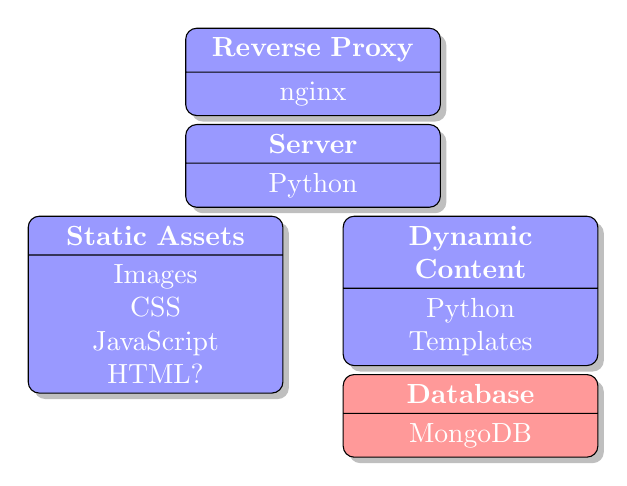
\begin{tikzpicture}[node distance=0.1cm]
        \node (proxy) [object, rectangle split, rectangle split parts=2]
        {
          \textbf{Reverse Proxy}
          \nodepart{second}nginx
        };
        \node (Server) [object, rectangle split, rectangle split parts=2, below=of proxy]
        {
          \textbf{Server}
          \nodepart{second}Python
        };
        \node (Frontend) [object, rectangle split, rectangle split parts=2, below=of Server, xshift=-2cm]
        {
          \textbf{Static Assets}
          \nodepart{second}Images \\ CSS \\ JavaScript \\ HTML?
        };
        \node (Backend) [object, rectangle split, rectangle split parts=2, below=of Server, xshift = 2cm]
        {
          \textbf{Dynamic Content}
          \nodepart{second}Python\\Templates
        };
        \node (Database) [highlight, rectangle split, rectangle split parts=2, below=of Backend]
        {
          \textbf{Database}
          \nodepart{second}MongoDB
        };
      \end{tikzpicture}
    \end{center}
\end{frame}

\begin{frame}
  \frametitle{Introducing MongoDB}
  \begin{figure}[h!]
    \centering
    
\includegraphics[scale=0.75]{imgs/mongodb_logo}
    \caption{MongoDB (from ``humongous'') is an open-source document database, and the leading NoSQL database.}
    \label{fig:mongodb}
  \end{figure}
\end{frame}

\begin{frame}
  \frametitle{NoSQL? Wat? --- A diversion on databases}
  \begin{itemize}
  \item Traditional database (e.g. MySQL ($\to$ MariaDB), PostgresSQL, MS-SQL) = Relational Databases
  \item ``NoSQL'' $\to$ umbrella term for a large number of non-relational databases.
    \begin{itemize}
    \item Document: e.g. MongoDB/CouchDB
    \item Key-value store: e.g. Redis
    \item Other exciting things: e.g. Neo4j - graph database, 
    \end{itemize}
  \end{itemize}

  Both are \emph{tools for different purposes}, with \emph{different
    strenghts and weaknesses}. \textbf{Just because MongoDB is cool,
    doesn't mean it is the solution to all your problems.}
\end{frame}

\begin{frame}
  \frametitle{Why MongoDB for us now?}
  \begin{itemize}
  \item Even with advanced database migration tools like South (for
    Django), it's still easier to do schema migrations in
    MongoDB. This helps with the sort of rapid prototyping we're doing here.
  \item It's really easy to store files/images in a
    MongoDB. Not necessarily super-efficient, but again good for
    prototyping.
  \item Often easier to wrap your head around.
  \end{itemize}
\end{frame}

\begin{frame}
  \frametitle{Getting started with MongoDB}

  \begin{itemize}
  \item Key component is a document.
  \item Document has a unique ID.
  \item Documents are JSON-like.
  \item Can contain arbitrary key-value pairs. Values can include
    arrays and other key-value mappings (`objects')
  \end{itemize}
\end{frame}

\begin{frame}[fragile]
\frametitle{An Example}
\begin{minted}{js}
{ "title" : "Post",
  "content" : "I think W, Y, and Z.",
  "author" : "Daniel Axtens",
  "date" : ISODate("2013-10-25T08:45:00Z"),
  "comments" : [{
    "author" : "Anonymous",
    "content" : "First P0000st!",
    "date" : ISODate("2013-09-25T10:01:44.405Z")
  }, {
    "author" : "Mr. Helpful",
    "content" : "I think you might have missed X, \
                which is listed on my blog.",
    "link" : "http://helpful.blog.com/",
    "date" : ISODate("2013-09-25T10:01:44.405Z")
  }]}
\end{minted}
\end{frame}

\begin{frame}[fragile]
  \frametitle{Converting this to code}

  Only chumps and people who enjoy getting owned write their own
  queries. We use MongoEngine. This is \texttt{blog\_example.py}:

  \inputminted[firstline=1,lastline=11]{python}{../steps/02-database/blog_example.py}
\end{frame}

\begin{frame}[fragile]
  Now, let's connect to the database, create and save a post. (This is
  more of \texttt{blog\_example.py})

  \inputminted[firstline=13,lastline=21]{python}{../steps/02-database/blog_example.py}
\end{frame}

\begin{frame}[fragile]
  \frametitle{Exploring your newly created document}
\begin{verbatim}
$ mongo
> use blog_example
> show collections
> db.blog_posts.find()
> db.blog_posts.find({'author': 'Daniel Axtens'})[0]
\end{verbatim}
SQL equivalent:
 \mint{sql}|SELECT * FROM blog_posts WHERE author = 'Daniel Axtens'|
\end{frame}

\begin{frame}
  \frametitle{Retriving with MongoEngine}
  \inputminted[firstline=22,lastline=35]{python}{../steps/02-database/blog_example.py}
\end{frame}

\begin{frame}[fragile]
  \frametitle{But I want my blog to have comments!}
  \inputminted[firstline=5,lastline=11]{python}{../steps/02-database/comment_example.py}
  \begin{minted}{python}
class BlogPost(Document):
    ...
    comments = ListField(EmbeddedDocumentField(Comment))    
  \end{minted}
\end{frame}

\begin{frame}
  \frametitle{But I want my blog to have comments!}
  \inputminted[firstline=33,lastline=44]{python}{../steps/02-database/comment_example.py}
\end{frame}

\begin{frame}
  \frametitle{But I want my blog to have comments!}
  \inputminted[firstline=46,lastline=59]{python}{../steps/02-database/comment_example.py}
\end{frame}

\begin{frame}
  \frametitle{But I want my blog to have comments!}
  \begin{itemize}
  \item Did you notice the seamless and painless schema migration?
  \item Did you notice the really, really painless Object-Document
    Mapping? Treating a list of comments as a Python list?
  \end{itemize}
\end{frame}

\begin{frame}
  \frametitle{Over to you...}
  \begin{itemize}
  \item What can a MongoEngine Document contain? (Highlights - see
    the online documentation for the full list)
    \begin{itemize}
    \item BooleanField
    \item DateTimeField
    \item IntField / LongField / DecimalField / FloatField
    \item DictField / MapField
    \item EmailField / URLField
    \item EmbeddedDocumentField
    \item FileField / ImageField
    \item GeoPointField
    \item ListField / SortedListField
    \item ReferenceField
    \item StringField
    \end{itemize}
  \item There's also an awesome inheritance system.
  \end{itemize}
\end{frame}

\begin{frame}
  \frametitle{Database}
    \begin{center}
      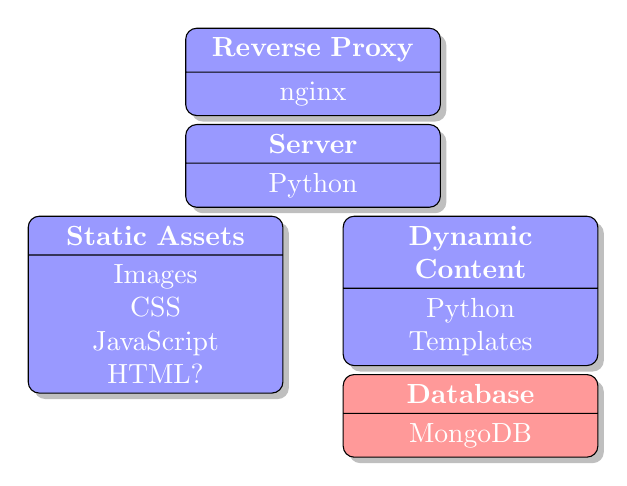
\begin{tikzpicture}[node distance=0.1cm]
        \node (proxy) [object, rectangle split, rectangle split parts=2]
        {
          \textbf{Reverse Proxy}
          \nodepart{second}nginx
        };
        \node (Server) [object, rectangle split, rectangle split parts=2, below=of proxy]
        {
          \textbf{Server}
          \nodepart{second}Python
        };
        \node (Frontend) [object, rectangle split, rectangle split parts=2, below=of Server, xshift=-2cm]
        {
          \textbf{Static Assets}
          \nodepart{second}Images \\ CSS \\ JavaScript \\ HTML?
        };
        \node (Backend) [object, rectangle split, rectangle split parts=2, below=of Server, xshift = 2cm]
        {
          \textbf{Dynamic Content}
          \nodepart{second}Python\\Templates
        };
        \node (Database) [highlight, rectangle split, rectangle split parts=2, below=of Backend]
        {
          \textbf{Database}
          \nodepart{second}MongoDB
        };
      \end{tikzpicture}
    \end{center}
\end{frame}

\begin{frame}
  \frametitle{Serving up your database}
    \begin{center}
      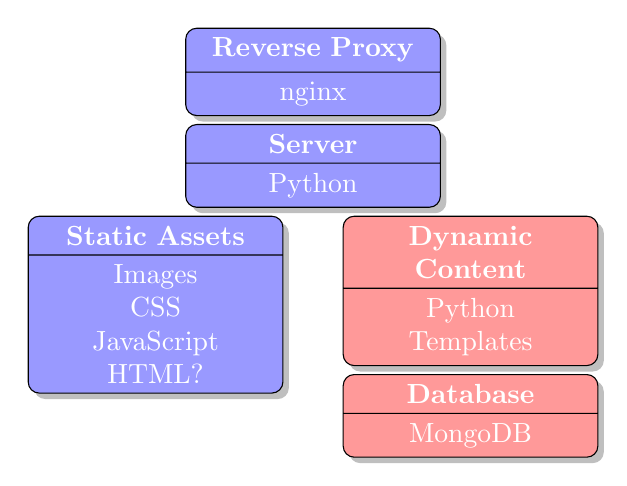
\begin{tikzpicture}[node distance=0.1cm]
        \node (proxy) [object, rectangle split, rectangle split parts=2]
        {
          \textbf{Reverse Proxy}
          \nodepart{second}nginx
        };
        \node (Server) [object, rectangle split, rectangle split parts=2, below=of proxy]
        {
          \textbf{Server}
          \nodepart{second}Python
        };
        \node (Frontend) [object, rectangle split, rectangle split parts=2, below=of Server, xshift=-2cm]
        {
          \textbf{Static Assets}
          \nodepart{second}Images \\ CSS \\ JavaScript \\ HTML?
        };
        \node (Backend) [highlight, rectangle split, rectangle split parts=2, below=of Server, xshift = 2cm]
        {
          \textbf{Dynamic Content}
          \nodepart{second}Python\\Templates
        };
        \node (Database) [highlight, rectangle split, rectangle split parts=2, below=of Backend]
        {
          \textbf{Database}
          \nodepart{second}MongoDB
        };
      \end{tikzpicture}
    \end{center}
\end{frame}

\begin{frame}
  \frametitle{Reading/Writing from your MongoDB}
  \begin{itemize}
  \item I usually put all my class definitions and my
    \texttt{connect(...)} call in a separate file
    (e.g. \texttt{database.py}), then say:
    
    \mint{python}|from database import *| 
    
    Although there's really no reason you couldn't have it all in one
    file. (Neatness concerns aside.)
  \end{itemize}
\end{frame}

\begin{frame}
  \frametitle{Simple and stupid example}
  \inputminted[firstline=8,lastline=22]{python}{../steps/02-database/01-webapp.py}
\end{frame}

\begin{frame}
  \frametitle{Off you go!}
  {\Huge Now work on the core of your own app! I'll be around if you
    have questions or need help.}
\end{frame}

\subsection{Front end}

\begin{frame}
  \frametitle{Front end}
    \begin{center}
      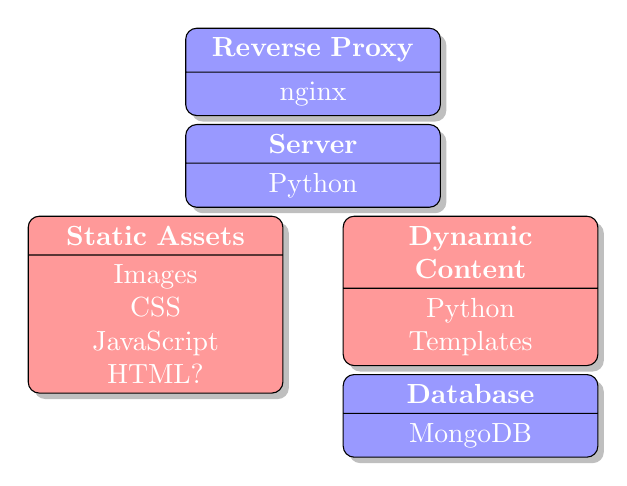
\begin{tikzpicture}[node distance=0.1cm]
        \node (proxy) [object, rectangle split, rectangle split parts=2]
        {
          \textbf{Reverse Proxy}
          \nodepart{second}nginx
        };
        \node (Server) [object, rectangle split, rectangle split parts=2, below=of proxy]
        {
          \textbf{Server}
          \nodepart{second}Python
        };
        \node (Frontend) [highlight, rectangle split, rectangle split parts=2, below=of Server, xshift=-2cm]
        {
          \textbf{Static Assets}
          \nodepart{second}Images \\ CSS \\ JavaScript \\ HTML?
        };
        \node (Backend) [highlight, rectangle split, rectangle split parts=2, below=of Server, xshift = 2cm]
        {
          \textbf{Dynamic Content}
          \nodepart{second}Python\\Templates
        };
        \node (Database) [object, rectangle split, rectangle split parts=2, below=of Backend]
        {
          \textbf{Database}
          \nodepart{second}MongoDB
        };
      \end{tikzpicture}
    \end{center}
\end{frame}

\begin{frame}
  \frametitle{Introducing Bootstrap}
  \begin{figure}[h!]
    \centering
    
\includegraphics[scale=0.3]{imgs/bootstrap_banner.png}
    \caption{Bootstrap: \url{getbootstrap.com}}
    \label{fig:bootstrap_banner}
  \end{figure}

  \begin{itemize}
  \item We're lazy, so we use Bootstrap for the frontend.
\end{itemize}
\end{frame}

\begin{frame}
  \frametitle{What can I do with Bootstrap?}
  \begin{itemize}
  \item Have things look not-terrible with minimal effort.
  \item Have mobile-compatible (``responsive'') layouts basically for
    free.
  \item Get a bunch of integrated client-side behaviours through
    jQuery.
  \item There are more things. (I cannot do design to save my life.)
  \end{itemize}
\end{frame}

\begin{frame}[fragile]
\frametitle{Setting up Bootstrap}
\begin{itemize}
\item Download it from \url{getbootstrap.com/getting-started}, extract
  the archive, put the folders in \texttt{static/}
  \begin{itemize}
  \item \emph{Don't download the version from the front page. Get the
      one with the pre-compiled JS and CSS assets.}
  \end{itemize}
  \item Choose the example from
    \url{http://getbootstrap.com/getting-started/#examples} that best
    suits your project.
    \begin{itemize}
      \item (Optionally) find it on GitHub.
      \item Copy the code to \texttt{views/index.tpl}
      \item Download any extra stylesheets, etc.
      \item Adjust relevant links to read \texttt{/static/\{js, css,
          etc\}/...} (look for \texttt{src=}, \texttt{href=})
      \item Fill out the relevant title, meta, etc tags.
    \end{itemize}
  \item Adjust your code to use the \texttt{index} template. Include
    your parameters (e.g. \texttt{\{\{name\}\}}) in there somewhere :)
  \end{itemize}
\end{frame}

\begin{frame}[fragile]
  \frametitle{But my submission page/other page/etc is still ugly!}
  \begin{itemize}
  \item You could copy-paste the template code. Or you could save
    yourself huge amounts of effort by being smart.
  \item Create \texttt{bootstrapbase.tpl}, and copy-paste the content
    of \texttt{index.tpl}.
  \item Delete everything from (and including):
\mint{html}|<div class="jumbotron">|
to (and not including):
\mint{html}|<div class="footer">|
Replacing it with the text \texttt{\%include}.
\item Title (replace Slogan Generator with your project name):
\mint{html}|<title>{{get('title', 'Slogan Generator')}}</title>|
\item Likewise with meta tags, you can pass them in as a variable if
  needed.
  \end{itemize}
\end{frame}

\begin{frame}
  \frametitle{But my submission page/other page/etc is still ugly!}
  \begin{itemize}
  \item Now back to \texttt{index.tpl}.
  \item Delete everything \emph{except} what we deleted from
    \texttt{bootstrapbase.tpl}
  \item At the top of \texttt{index.tpl} add:\\
    \texttt{\%rebase bootstrapbase}
  \end{itemize}
\end{frame} 

\begin{frame}
  \frametitle{Contacts page}
  \texttt{webapp.py}:
  \inputminted[firstline=34,lastline=38]{python}{../steps/03-frontend/02-demo-app/webapp.py}
  \texttt{views/contact.tpl}:
  \inputminted{html}{../steps/03-frontend/02-demo-app/views/contact.tpl}
\end{frame}

\begin{frame}
  \begin{itemize}
  \item This doesn't deal correctly with the highlighting in the top
    bar. This is a bit fiddly so I'm not going to go through it
    now. Some sample code is included, however.
  \item As things start to get more complicated (replacing chunks of
    different pages), it's time to swap out SimpleTemplate for a less
    simple system (e.g. Jinja). (It's possibly also time to move to a
    more comprehensive framework.)
  \end{itemize}
\end{frame}

\begin{frame}
  \frametitle{Buzzword time: AJAX}
  \begin{itemize}
  \item AJAX stands for Asynchronous JavaScript and XML.
  \item That's not how the term is used any more, however.
    \begin{itemize}
    \item JSON (JavaScript Object Notation) $>>$ XML (eXtensible
      Markup Language)
    \item It can also be synchronous.
    \item Umbrella term for ``getting stuff from a server without
      loading an entire page again''.
    \end{itemize}
  \item jQuery (which comes for free with Bootstrap) makes AJAX
    painless. {\tiny ... or at least as painless as something in JavaScript can be.}
  \end{itemize}
\end{frame}

\begin{frame}[fragile]
  \frametitle{AJAX: JSON}
  \begin{itemize}
  \item JSON is awesome. We've seen it before with MongoDB. It is also
    the way JavaScript expresses objects.
  \item Key-value, \texttt{\{...\}} for objects, \texttt{[...]} for
    arrays.
  \item Trivial to parse and generate in every useful language! (Don't
    DIY it, and especially don't use JS's eval function on it.)
  \item Lets make our server spit out JSON!
  \end{itemize}
\end{frame}

\begin{frame}[fragile]
  \frametitle{Back to \texttt{webapp.py}}
  \begin{itemize}
  \item \mint{python}|from bottle import route, run, ..., response| 
  \item \mint{python}|import json|
  \item \inputminted[firstline=21,lastline=25]{python}{../steps/03-frontend/04-demo-app/webapp.py}
  \end{itemize}
\end{frame}

\begin{frame}
  \frametitle{Front end: Introducing jQuery}
  \begin{figure}[h!]
    \centering
    
\includegraphics{imgs/jquery_logo}
    \caption{jQuery --- write less, do more. \url{http://jquery.com}}
    \label{fig:jquery}
  \end{figure}
  \begin{itemize}
  \item jQuery makes JavaScript in the browser not suck.
  \item I heart it immensely.
  \end{itemize}
\end{frame}

\begin{frame}
  \frametitle{Front end---\texttt{index.tpl}}
  \begin{itemize}
  \item (These will probably be different for you. I'll run through it
    and then be around to help.)
  \item Add \texttt{id="slogan"} to the \texttt{h1} with
    \texttt{\{\{slogan\}\}}.
  \item Add \texttt{id="generate"} to the \texttt{a} with
    \texttt{role="button"}. If you've changed the \texttt{href},
    change it back to \texttt{\#}.
  \end{itemize}
\end{frame}

\begin{frame}
  \frametitle{Front end---\texttt{static/js/ajax.js}}
  \inputminted{js}{../steps/03-frontend/04-demo-app/static/js/ajax.js}
\end{frame}

\begin{frame}[fragile]
  \frametitle{Including the script---a bit of hackery in
    \texttt{bootstrapbase.tpl}}
  
  After the other scripts:
  \begin{minted}{html}
       <script src="/static/js/ajax.js"></script>
  \end{minted}

  Yes, this isn't particularly extensible. But jQuery falls over
  nicely.
\end{frame}

\begin{frame}
  \frametitle{Hurray, AJAX!}

  \texttt{Don't forget to save to git!}
\end{frame}

\begin{frame}
  \frametitle{A review: what have we done?}
  \begin{itemize}
  \item A web server written in Python...
  \item ... reading and writing data from MongoDB ...
  \item ... with a front end made less ugly by Bootstrap ...
  \item ... with interactivity through AJAX, implemented in jQuery...
  \item ... running in a virtual machine on your computer.
  \end{itemize}
\end{frame}

\section{Deploying your app!}

\begin{frame}
  \frametitle{Deploying your app!}
  \begin{itemize}
  \item As exciting as virtual machines on your computer are...
  \item ... virtual machines on someone else's computer are cooler ...
  \item ... especially when that other computer is permanently
    connected to the internet.
  \end{itemize}
\end{frame}

\begin{frame}
  \frametitle{One small thing...}
  Take out \texttt{debug=True, reloader=True} from \texttt{webapp.py}.
\end{frame}

\begin{frame}
  \frametitle{Re-introducing AWS}
  \begin{figure}[h!]
    \centering
    
\includegraphics[scale=0.4]{imgs/aws_logo.png}
    \caption{Amazon Web Services delivers a set of services that together form a reliable, scalable, and inexpensive computing platform ``in the cloud''. \url{aws.amazon.com}}
    \label{fig:aws_logo}
  \end{figure}

  {\tiny ``Amazon Web Services'' and the ``Powered by Amazon Web
    Services'' logo, are trademarks of Amazon.com, Inc. or its
    affiliates in the United States and/or other countries.}
\end{frame}

\begin{frame}[fragile]
  \frametitle{Somewhere to put your code}

  \aws{sudo adduser --disabled-password webapp}

\end{frame}

\begin{frame}
  \frametitle{Getting your source code to the server: introducing
    Fabric}

  \begin{quote}
  Fabric is a Python (2.5 or higher) library and command-line tool for
  streamlining the use of SSH for application deployment or systems
  administration tasks.
  \end{quote}

  \url{http://fabfile.org}

\end{frame}

\begin{frame}
  \frametitle{\texttt{fabfile.py}}
  \inputminted{python}{../steps/04-deployment/01-demo-app/fabfile.py}
\end{frame}

\begin{frame}
  \frametitle{Let's go!}
  \begin{itemize}

  \item \aws{sudo apt-get -y install python-pip python-dev mongodb}

  \item \texttt{fab -u ubuntu -H \textit{number}.compcon.dja.id.au
      setup}
  \item \texttt{fab -u ubuntu -H \textit{number}.compcon.dja.id.au deploy}

  \item \aws{sudo -u webapp -s}\\
    \aws{python webapp.py}
  
  \item Your code should be running, but the website won't work on
    port 80, and 8080 is firewalled off.

  \end{itemize}
\end{frame}

\begin{frame}
  \frametitle{What not to do}
  \begin{itemize}
  \item<1-> ``Why don't we just set \texttt{port=80} in the \texttt{run}
    function call?''
  \item<2-> ``Oh, that's odd, it can't bind to port 80. Oh, it's a
    privileged port? Oh, I can just run it as root!''
  \item<3-> ``Yay, it works now!''
  \item<4-> $<$ring ring$>$ ``Hello, this is developer'' ... ``What do
    you mean my app got owned? My server got owned? And wiped out
    everything else on the server?''
  \end{itemize}
\end{frame}

\begin{frame}
  \frametitle{What not to do}
  {\Huge Don't run your app as root. Ever. Not even for a little
    while.}
\end{frame}

\begin{frame}
  \frametitle{Introducing our saviour ... nginx}
  \begin{figure}[h!]
    \centering
    
\includegraphics[scale=0.4]{imgs/nginx_logo.png}
    \caption{nginx}
    \label{fig:nginx_logo}
  \end{figure}
  \begin{itemize}
  \item \aws{sudo apt-get -y install nginx-light}
  \end{itemize}
\end{frame}

\begin{frame}
  \frametitle{Reverse Proxy}
    \begin{center}
      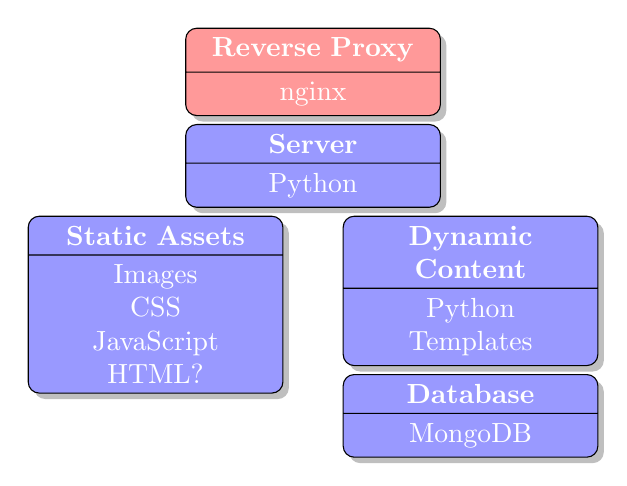
\begin{tikzpicture}[node distance=0.1cm]
        \node (proxy) [highlight, rectangle split, rectangle split parts=2]
        {
          \textbf{Reverse Proxy}
          \nodepart{second}nginx
        };
        \node (Server) [object, rectangle split, rectangle split parts=2, below=of proxy]
        {
          \textbf{Server}
          \nodepart{second}Python
        };
        \node (Frontend) [object, rectangle split, rectangle split parts=2, below=of Server, xshift=-2cm]
        {
          \textbf{Static Assets}
          \nodepart{second}Images \\ CSS \\ JavaScript \\ HTML?
        };
        \node (Backend) [object, rectangle split, rectangle split parts=2, below=of Server, xshift = 2cm]
        {
          \textbf{Dynamic Content}
          \nodepart{second}Python\\Templates
        };
        \node (Database) [object, rectangle split, rectangle split parts=2, below=of Backend]
        {
          \textbf{Database}
          \nodepart{second}MongoDB
        };
      \end{tikzpicture}
    \end{center}
\end{frame}


\begin{frame}[fragile]
  \frametitle{\aws{sudo nano /etc/nginx/sites-available/default}}

\begin{verbatim}
server {
        server_name NUMBER.compcon.dja.id.au;

        location / {
                proxy_pass http://localhost:8080/;
        }
}
\end{verbatim}

  \begin{itemize}
  \item \aws{sudo service nginx restart}
  \item Start your process and (assuming it doesn't rely on a
    pre-seeded database!) it should work!
  \end{itemize}
\end{frame}

\begin{frame}
  \frametitle{``Staying alive, staying alive''\\Introducing
    \texttt{supervisord}}
  \begin{figure}[h!]
    \centering
    
\includegraphics{imgs/supervisord_logo}
    \caption{Supervisord: hang on to your processes. \url{http://supervisord.org} }
    \label{fig:supervisord_logo}
  \end{figure}

  \begin{itemize}
  \item \aws{sudo apt-get -y install supervisor}
  \end{itemize}
  
\end{frame}

\begin{frame}[fragile]
  \frametitle{\aws{sudo nano /etc/supervisord/conf.d/webapp.conf}}
\begin{verbatim}
[program:webapp]
user=webapp
command=python /home/webapp/webapp.py
autostart=true
autorestart=true
\end{verbatim}
  \aws{sudo service supervisor stop; sudo service supervisor start;}
\end{frame}

\begin{frame}[fragile]
  \frametitle{Oh no, it's b0rked!}

  \begin{itemize}
  \item<1-> \texttt{webapp.py}: 
\begin{minted}{python}
if root:
    os.chdir(root)
\end{minted}
  \item<2-> \texttt{fab -u ubuntu -H \textit{number}.compcon.dja.id.au
      deploy}
  \item<2-> \aws{sudo supervisorctl restart webapp}
  \item<3-> (even better, add the following to \texttt{fabfile.py})
\mint{python}|sudo("supervisorctl restart webapp")|
  \end{itemize}
\end{frame}

\begin{frame}
  \frametitle{Recap}
    \begin{center}
      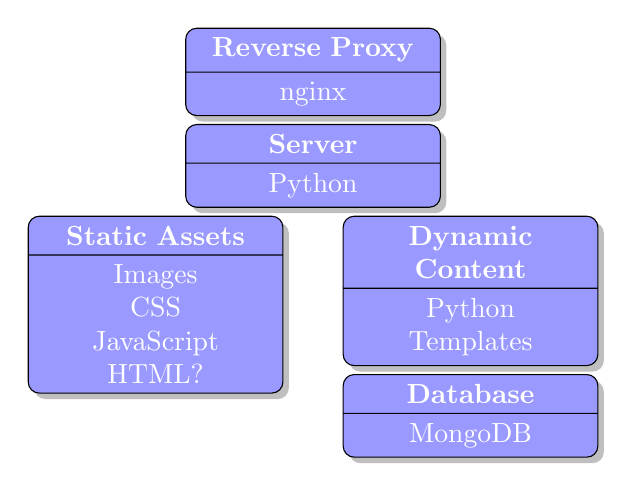
\begin{tikzpicture}[node distance=0.1cm]
        \node (proxy) [object, rectangle split, rectangle split parts=2]
        {
          \textbf{Reverse Proxy}
          \nodepart{second}nginx
        };
        \node (Server) [object, rectangle split, rectangle split parts=2, below=of proxy]
        {
          \textbf{Server}
          \nodepart{second}Python
        };
        \node (Frontend) [object, rectangle split, rectangle split parts=2, below=of Server, xshift=-2cm]
        {
          \textbf{Static Assets}
          \nodepart{second}Images \\ CSS \\ JavaScript \\ HTML?
        };
        \node (Backend) [object, rectangle split, rectangle split parts=2, below=of Server, xshift = 2cm]
        {
          \textbf{Dynamic Content}
          \nodepart{second}Python\\Templates
        };
        \node (Database) [object, rectangle split, rectangle split parts=2, below=of Backend]
        {
          \textbf{Database}
          \nodepart{second}MongoDB
        };
      \end{tikzpicture}
    \end{center}
\end{frame}

\section{Further directions}

\begin{frame}
  \frametitle{Further directions}
  \begin{itemize}
  \item If you're still sorting out bugs, etc., keep working on that.
  \item If not, here's some stuff we can look at adding:
    \begin{itemize}
    \item Google Analytics
    \item Authentication
    \item Speed improvements
    \item CloudFlare
    \end{itemize}
  \end{itemize}
\end{frame}

\begin{frame}
  \frametitle{Introducing Google Analytics}
  \begin{figure}[h!]
    \centering
    
\includegraphics[scale=0.3]{imgs/ga_logo}
    \caption{Google Analytics: Turning data insights into action. \url{http://google.com/analytics}}
    \label{fig:ga_logo}
  \end{figure}

  You can figure this out yourself. Just copy the snippet into \texttt{bootstrapbase.tpl}.
  
\end{frame}

\begin{frame}
  \frametitle{Authentication}
  \begin{itemize}
  \item<1-> We probably don't have time to cover this properly.
  \item<2-> (Daniel rants about security.)
  \item<3-> Introducing Cork.
  \item<4-> Seriously consider a more heavy-weight framework.
  \end{itemize}
\end{frame}

\begin{frame}
  \frametitle{``You are not done yet''}
  \begin{itemize}
  \item Your site is slow. \texttt{nginx} can make it faster with
    gzipping, caching and by retrieving assets without going through
    Bottle.
  \item Bottle is slow because it uses a reference WSGI server. Try
    CherryPy or Paste.
  \item Consider CloudFlare.
  \item Consider accessibility.
  \end{itemize}
\end{frame}

\begin{frame}
  \frametitle{Bonus: ``With great power comes great
    responsibility''\\Introducing Boto}
  
  \begin{itemize}
  \item ``I have a workshop coming up where I want 30 people to have
    virtual machines with custom DNS names. Setting up each one takes
    a couple of minutes and I am very, very lazy.''
  \end{itemize}

\end{frame}

\end{document}
